\chapter{REFERENCIAL TEÓRICO}

Este capítulo apresenta os principais conceitos teóricos que fundamentam o desenvolvimento desta pesquisa. 
Inicialmente, são introduzidos os fundamentos de AM, destacando suas principais características e aplicações no contexto da modelagem preditiva. 
Na sequência, são abordados conceitos de PO, com ênfase em problemas de otimização combinatória e em métodos heurísticos que servem de base à 
abordagem de otimização da composição de elencos proposta neste trabalho.

\section{Aprendizado de Máquina (AM)}

Aprendizado de Máquina (AM) é o estudo de algoritmos e modelos estatísticos empregados por sistemas computacionais para realizar tarefas específicas de forma autônoma. 
Essa abordagem permite que as máquinas aprendam a partir de dados e melhorem seu desempenho sem necessidade de reprogramação explícita \cite{Mahesh2020}. 
Segundo Geron (2019), AM pode ser descrito como a ciência (ou arte) de programar computadores para que aprendam com os dados.

Um exemplo clássico de aplicação de AM é o filtro de \textit{spam}, que permite que o sistema identifique automaticamente emails indesejados, 
diferenciando-os de mensagens legítimas com base em padrões aprendidos \cite{Geron2019}. 

Com a crescente disponibilidade de \textit{datasets}, o uso de AM tem apresentado um notável crescimento \cite{Mahesh2020}. 
Esse avanço pode ser atribuído à maior disponibilidade de dados e ao aumento da capacidade computacional. 
A constante conexão das pessoas a dispositivos digitais gera volumes massivos de dados, enquanto tecnologias modernas permitem o 
processamento eficiente dessas grandes quantidades de informação \cite{Jordan2015}.

Muitas indústrias têm adotado o AM com o objetivo de extrair insights relevantes de \textit{databases}, facilitando o aprendizado a partir dos dados \cite{Mahesh2020}. 
Além disso, o AM tem sido amplamente aplicado em diversas áreas, incluindo reconhecimento facial, segmentação de imagens, detecção de câncer e previsão de classes 
e resultados, destacando-se também no contexto esportivo \cite{Almulla2023}.

No desenvolvimento de sistemas de AM, a construção de modelos geralmente ocorre dentro de um pipeline composto por múltiplas etapas de processamento de dados. 
Em um projeto típico de AM, os dados passam inicialmente por fases de coleta e preparação, seguidas por etapas de exploração e preparação dos dados, 
engenharia de atributos, seleção e treinamento de modelos, além de procedimentos de avaliação e ajuste de hiperparâmetros \cite{Geron2019}. 
Essas etapas são frequentemente organizadas em forma de pipeline, no qual cada componente executa uma transformação específica sobre os dados 
e produz uma saída que será utilizada pela etapa subsequente do processo \cite{Geron2019}. 
Essa estrutura modular permite organizar o fluxo de processamento e facilita a reprodução e manutenção dos modelos desenvolvidos. 
Um exemplo de organização dessas etapas no ciclo de vida de um projeto de análise de dados é apresentado na Figura \ref{fig:crispdm_pipeline}, 
baseada no processo CRISP-DM, amplamente utilizado em projetos de mineração de dados e AM \cite{Kelleher2015}.

\begin{figure}[H]
\centering
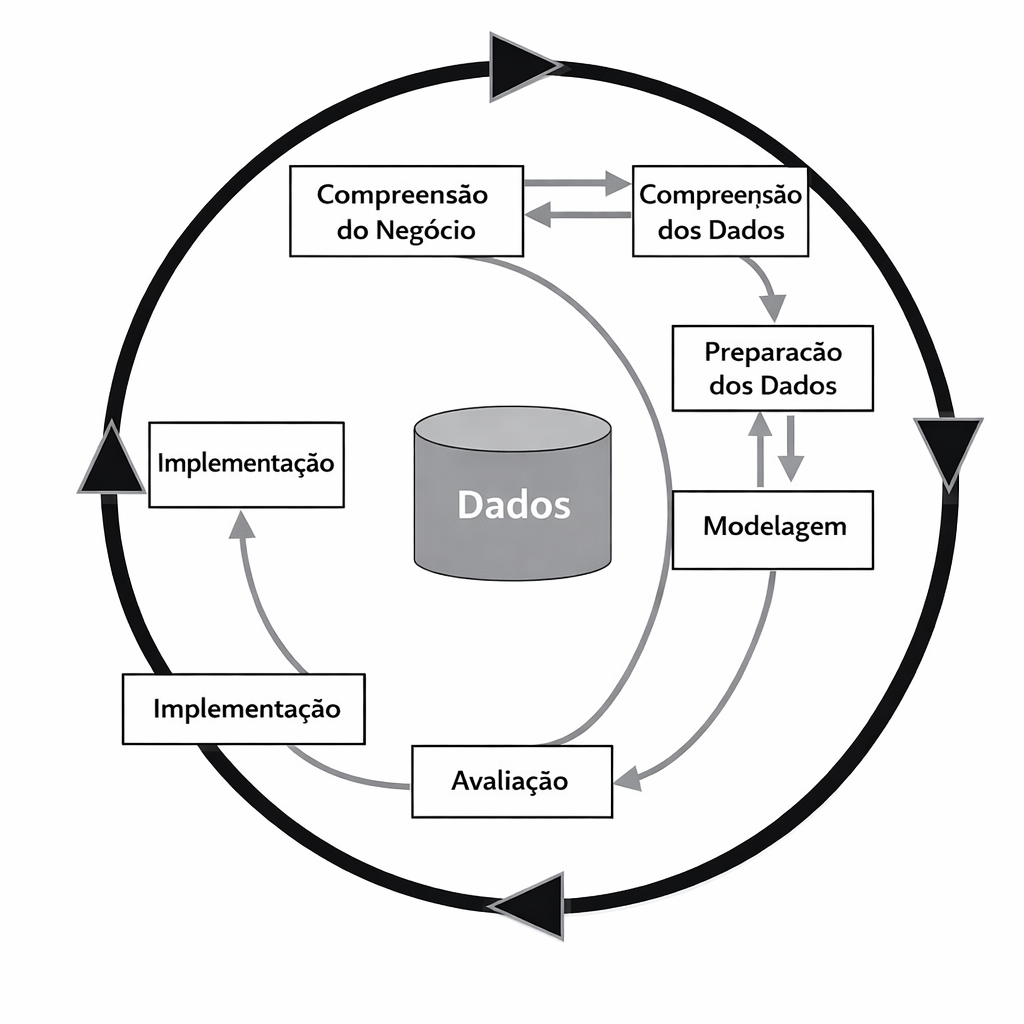
\includegraphics[width=0.8\textwidth]{imagens/ml-pipeline.png}
\caption{Pipeline CRISP-DM}
\label{fig:crispdm_pipeline}
{\footnotesize Fonte: Adaptado de \cite{Kelleher2015}.}
\end{figure}

Dentro desse pipeline, a preparação e transformação dos dados desempenham papel fundamental, 
uma vez que os algoritmos de aprendizado frequentemente exigem representações específicas dos atributos para funcionar adequadamente.

\subsection{Generalização, Viés e Variância}

Um dos principais desafios em AM é garantir que o modelo apresente boa capacidade de generalização, isto é, desempenho satisfatório em dados não 
utilizados durante o treinamento \cite{Goodfellow2016}. 

Modelos excessivamente complexos podem se ajustar não apenas aos padrões relevantes, mas também ao ruído presente no conjunto de treinamento, 
fenômeno conhecido como \textit{overfitting}. Em contrapartida, modelos demasiadamente simples podem não capturar relações importantes nos dados, 
resultando em \textit{underfitting}.

Esse comportamento está diretamente relacionado ao equilíbrio entre viés e variância. Modelos com alto viés tendem a apresentar subajuste, enquanto 
modelos com alta variância tornam-se excessivamente sensíveis às particularidades do conjunto de treinamento. Técnicas como validação cruzada, regularização 
e controle da complexidade do modelo são estratégias amplamente utilizadas para mitigar esses problemas \cite{Geron2019}.

\subsection{Seleção de Atributos e Redução de Dimensionalidade}

Em problemas com elevado número de variáveis explicativas, a presença de atributos redundantes ou irrelevantes pode impactar negativamente 
o desempenho dos modelos preditivos. A seleção de atributos busca identificar subconjuntos de variáveis que contribuam de forma significativa para 
a tarefa de aprendizagem \cite{Liu2010}.

Os métodos de seleção podem ser classificados em três categorias principais: filtros, que utilizam medidas estatísticas independentes do modelo; 
wrappers, que avaliam subconjuntos de atributos com base no desempenho de um algoritmo específico; e métodos embutidos, nos quais a seleção ocorre 
durante o próprio processo de treinamento \cite{Guyon2006}.

Além da seleção direta de atributos, técnicas de redução de dimensionalidade, como a Análise de Componentes Principais (PCA), 
realizam uma transformação linear das variáveis originais em um novo conjunto de componentes ortogonais que preservam a maior parte da variância dos dados. 
Essa abordagem pode reduzir complexidade computacional e mitigar problemas de multicolinearidade. Cabe ressaltar que a PCA não consiste em um método 
de seleção de atributos, mas sim em uma técnica de extração de atributos, pois cria novas variáveis a partir de combinações lineares das variáveis originais \cite{Guyon2006}.

Além dos aspectos relacionados à preparação e transformação dos dados, também é importante distinguir os principais paradigmas de 
aprendizagem utilizados na construção de modelos preditivos. Em AM, os algoritmos podem ser classificados em diferentes categorias de acordo com a forma 
como aprendem a partir dos dados. Uma das distinções mais comuns ocorre entre aprendizado supervisionado e não supervisionado. 
No aprendizado supervisionado, o modelo é treinado a partir de um conjunto de dados rotulados, no qual cada instância possui uma variável alvo associada. 
O objetivo do algoritmo é aprender uma função que relacione os atributos de entrada com essa variável alvo, permitindo realizar previsões para novas instâncias \cite{Geron2019}. 
Por outro lado, no aprendizado não supervisionado os dados não possuem rótulos explícitos, e o objetivo do algoritmo consiste em identificar padrões, estruturas ou agrupamentos 
presentes nos dados \cite{Geron2019}. Técnicas como \textit{clustering} e redução de dimensionalidade, incluindo a Análise de Componentes Principais (PCA), 
são exemplos de métodos amplamente utilizados nesse contexto.

Em problemas de aprendizado supervisionado, as tarefas podem ser geralmente divididas em classificação e regressão. Na classificação, o objetivo é atribuir 
cada instância a uma classe discreta previamente definida, como por exemplo identificar se um e-mail é \textit{spam} ou não \cite{Geron2019}. 
Já na regressão, busca-se prever valores numéricos 
contínuos a partir de um conjunto de variáveis explicativas, como a previsão de preços, temperaturas ou outras 
quantidades mensuráveis \cite{Geron2019}. No contexto deste trabalho, o problema é formulado como uma tarefa de regressão, 
uma vez que o objetivo consiste em estimar a pontuação final de equipes em um campeonato a partir das características 
individuais dos jogadores que compõem o elenco.

Após as etapas de preparação, transformação e possível redução de dimensionalidade dos dados, diferentes algoritmos de AM podem ser 
empregados para construir modelos preditivos. A seguir, são apresentados alguns dos algoritmos mais comumente utilizados para a resolução de problemas de 
regressão, abordagem adotada no modelo proposto neste trabalho.

Entre os diversos algoritmos disponíveis na literatura, foram selecionados neste trabalho métodos amplamente utilizados em aprendizado supervisionado 
para tarefas de regressão, incluindo modelos lineares, métodos baseados em árvores, métodos de \textit{boosting} e redes neurais artificiais.

\subsection{Regressão Linear (RL)}

A regressão linear é uma técnica estatística amplamente utilizada para investigar e modelar a relação entre variáveis, sendo aplicada em diversas áreas da ciência, 
engenharia e ciências sociais \cite{Montgomery2012}. Nesse método, assume-se que a variável dependente pode ser expressa como uma combinação 
linear das variáveis explicativas.

Na forma mais geral, a RL pode ser expressa como:

\begin{equation}
\hat{y} = \beta_0 + \beta_1 x_1 + \beta_2 x_2 + \dots + \beta_p x_p
\end{equation}

em que $\hat{y}$ representa o valor previsto da variável resposta, $\beta_0$ é o intercepto do modelo, $\beta_1, \beta_2, \dots, \beta_p$ são os coeficientes 
associados às variáveis explicativas e $x_1, x_2, \dots, x_p$ representam os atributos de entrada.

O processo de treinamento da RL consiste em estimar os coeficientes do modelo de forma a minimizar o erro entre os valores previstos e os valores observados no 
conjunto de treinamento. Uma abordagem amplamente utilizada para esse ajuste é o método dos mínimos quadrados ordinários, que busca minimizar a soma 
dos quadrados dos resíduos \cite{Geron2019}. Dessa forma, o modelo encontra a combinação linear dos atributos que melhor se ajusta aos dados segundo esse critério.

A RL apresenta como principais vantagens a simplicidade, a interpretabilidade e o baixo custo computacional. Por se tratar de um modelo linear, seus 
coeficientes podem ser interpretados como a contribuição de cada variável explicativa para a previsão da variável alvo, mantidas constantes as demais variáveis. 
Além disso, a RL costuma servir como modelo de referência (\textit{baseline}) em tarefas preditivas, permitindo comparar o 
desempenho de modelos mais complexos \cite{Geron2019}.

Entretanto, a RL possui limitações importantes, especialmente quando a relação entre as variáveis explicativas e a variável resposta não pode ser adequadamente 
representada por uma função linear. Nesses casos, o modelo tende a apresentar desempenho inferior ao de métodos capazes de capturar padrões não lineares mais complexos. 
Ainda assim, sua utilização permanece relevante tanto pela simplicidade quanto pelo seu papel como ponto de comparação em estudos de modelagem preditiva \cite{Geron2019}.

\subsection{Árvore de Decisão (AD)}

As Árvores de Decisão são algoritmos versáteis de AM que podem ser utilizados tanto para tarefas de classificação, quanto para tarefas de regressão \cite{Geron2019}. 
Esses algoritmos recebem dados de treinamento e retornam como saída uma estrutura em árvore capaz de realizar previsões para novas instâncias 
com base nos atributos de entrada \cite{Geron2019}.

A construção de uma árvore de decisão ocorre por meio de um processo recursivo de particionamento do espaço de atributos. Em cada nó interno da árvore, 
o algoritmo seleciona um atributo e um ponto de divisão que melhor separam os dados de acordo com um critério de qualidade da partição. 
Em tarefas de classificação, critérios como índice de Gini e entropia são amplamente utilizados, enquanto em problemas de regressão são comuns medidas 
baseadas na redução da variância ou do erro quadrático \cite{Geron2019}.

Além do processo de divisão recursiva, a geração de uma árvore de decisão envolve a escolha sucessiva dos melhores atributos e pontos de corte 
que maximizam a qualidade das partições geradas. Durante o treinamento, o algoritmo avalia diferentes possíveis divisões nos atributos disponíveis 
e seleciona aquela que produz o maior ganho de informação, a maior redução do índice de Gini ou a maior redução da variância/erro quadrático, 
dependendo da natureza do problema e do critério adotado. Esse procedimento é repetido de forma recursiva até que uma condição de parada seja satisfeita, 
como a profundidade máxima da árvore, o número mínimo de amostras em um nó ou a ausência de melhoria significativa na qualidade dos subconjuntos \cite{Geron2019}.

Em comparação com outras técnicas de aprendizado supervisionado, as árvores de decisão apresentam algumas características importantes. 
Uma de suas principais vantagens é a interpretabilidade, uma vez que a estrutura da árvore permite interpretar de forma transparente como as decisões são tomadas a partir 
dos atributos de entrada. Além disso, esses modelos requerem pouca preparação dos dados, pois não exigem normalização ou padronização das variáveis. Por outro lado, 
árvores de decisão individuais tendem a apresentar alta variância, sendo sensíveis a pequenas variações nos dados de treinamento. Essa característica pode levar 
ao fenômeno de \textit{overfitting}, motivo pelo qual métodos baseados em conjuntos de árvores, como o Random Forest, são frequentemente utilizados para 
melhorar a capacidade de generalização do modelo \cite{Geron2019}.

Um exemplo de AD pode ser visto na Figura~\ref{fig2_1}. 

\begin{figure}[h]
    \centering
    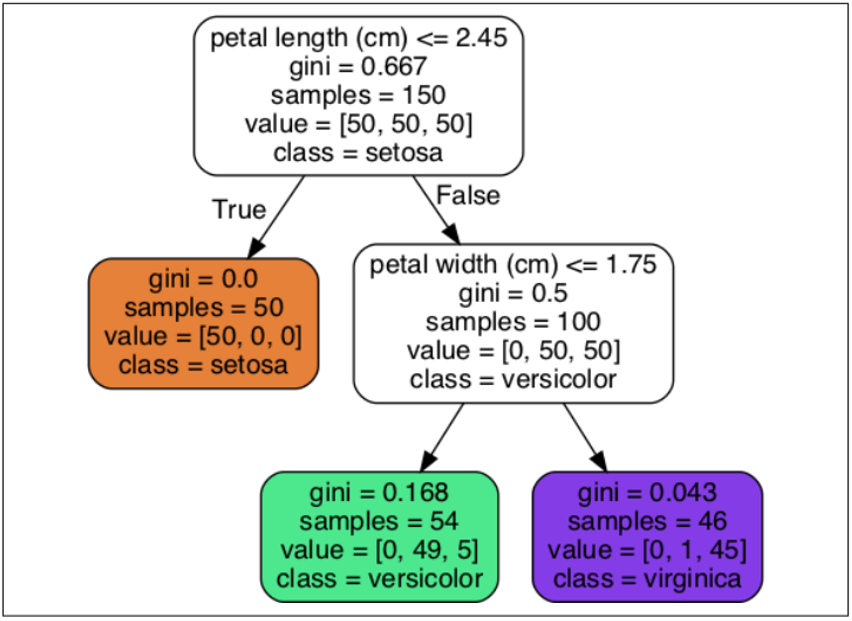
\includegraphics[width=1.0\linewidth]{imagens/ad_01.png}
    \caption{AD para Iris}
    {\small Fonte: Geron, 2019}
    \label{fig2_1}
\end{figure}

Na Figura~\ref{fig2_1}, é possível observar uma árvore de decisão utilizada para classificar flores do conjunto de dados \textit{Iris}. 
O nó raiz divide as amostras com base no comprimento da pétala (\textit{petal length} $\leq$ 2.45), separando a classe \textit{setosa} (pura, Gini = 0). 
As amostras restantes são subdivididas pelo critério de largura da pétala (\textit{petal width} $\leq$ 1.75), onde as classes \textit{versicolor} e \textit{virginica} 
são diferenciadas com alta precisão (Gini próximo de 0 nos nós finais). A árvore otimiza a classificação minimizando o índice de Gini em cada divisão \cite{Geron2019}. 

\subsection{Random Forest (RF)}

O RF consiste em uma combinação de AD, geralmente treinadas por meio do método \textit{bagging} \cite{Geron2019}. Diferente das ADs, RF 
utiliza uma randomização extra no crescimento das árvores. Ao invés de buscar a melhor \textit{feature} para dividir o nó, 
utiliza-se da melhor dentro de um \textit{subset} randômico. Nesse caso, busca-se reduzir a variância do modelo por meio da agregação de 
múltiplas árvores, mantendo um viés relativamente baixo quando comparado a modelos excessivamente regularizados.

A motivação para essa estratégia está relacionada à redução da variância do modelo. ADs individuais são modelos de alta variância, 
ou seja, pequenas variações no conjunto de treinamento podem resultar em estruturas de árvore significativamente diferentes. Ao treinar múltiplas 
árvores em subconjuntos distintos dos dados e introduzir aleatoriedade na seleção de atributos, o RF reduz a correlação entre os modelos 
individuais. Como consequência, ao combinar as previsões das árvores, os erros individuais tendem a se compensar, produzindo um modelo mais estável 
e com melhor capacidade de generalização quando comparado a uma única AD \cite{Geron2019}.

Além da seleção aleatória de subconjuntos de atributos em cada divisão, o RF também utiliza amostragem com reposição (\textit{bootstrap sampling}) para 
gerar diferentes subconjuntos de dados de treinamento para cada árvore. Esse procedimento, conhecido como \textit{bootstrap aggregating} 
ou \textit{bagging}, contribui para aumentar a diversidade entre os modelos individuais da floresta \cite{Geron2019}. 

Durante a fase de predição, as saídas das árvores são agregadas para produzir o resultado final do modelo. Em tarefas de classificação, 
essa agregação ocorre por meio de votação majoritária entre as árvores, enquanto em problemas de regressão o resultado é geralmente obtido pela 
média das previsões individuais \cite{Geron2019}. Essa estratégia reduz a variância do modelo e tende a melhorar a capacidade de generalização quando comparada 
ao uso de uma única AD.

\begin{comment}
\subsection{Support Vector Machine (SVM)}

O \textit{Support Vector Machine} (SVM) é um algoritmo de AM supervisionado utilizado para tarefas de classificação e regressão. 
Em sua formulação clássica de classificação, o objetivo consiste em encontrar um hiperplano ótimo que separe os dados em diferentes classes, 
maximizando a margem entre os pontos mais próximos das classes opostas \cite{noble2006}.

O hiperplano utilizado pelo SVM consiste em uma superfície de decisão que separa os pontos de dados em classes distintas. Em um espaço 2D, 
ele é uma linha; em 3D, um plano e, em dimensões superiores, uma hiper-superfície \cite{noble2006}.

Cabe ressaltar que nem sempre os dados são linearmente separáveis. Sendo assim, o SVM utiliza funções \textit{kernel} para projetar os 
dados em um espaço de maior dimensão, onde a separação linear se torna possível \cite{noble2006}. As principais funções \textit{kernel} são:

\begin{enumerate}
    \item \textbf{Linear}: Quando os dados já são linearmente separáveis.
    \item \textbf{Polinomial}: Para capturar relações não lineares.
    \item \textbf{RBF (Radial Basis Function - Gaussiana)}: Amplamente usada para capturar padrões complexos.
    \item \textbf{Sigmoid}: Similar a redes neurais.
\end{enumerate}

Além de tarefas de classificação, o SVM também pode ser aplicado a problemas de regressão, formulação conhecida como \textit{Support Vector Regression} (SVR). 
Nesse caso, o objetivo não consiste em separar classes, mas em encontrar uma função que aproxime os dados de treinamento com erro máximo limitado 
por um parâmetro de tolerância, geralmente representado por $\epsilon$. O modelo busca ajustar uma função que permaneça dentro de uma região de erro aceitável, 
ao mesmo tempo em que maximiza a margem em torno dessa função, preservando as propriedades de regularização do método \cite{Geron2019}.
\end{comment}
\subsection{Gradient Boosting (XGBoost)}

O \textit{Gradient Boosting} é uma técnica de aprendizado baseada na combinação sequencial de modelos fracos, geralmente árvores de decisão rasas, 
com o objetivo de minimizar uma função de perda diferenciável \cite{Geron2019}. Diferentemente do \textit{bagging}, no qual os modelos são treinados 
de forma independente, o \textit{boosting} constrói cada novo preditor de maneira iterativa, ajustando-o aos resíduos (erros) cometidos pelo modelo anterior. 
Esse processo pode ser interpretado como uma otimização por gradiente no espaço funcional, na qual cada novo modelo 
aproxima a direção de maior redução da função de custo.

Formalmente, a cada iteração \( m \), busca-se adicionar um novo modelo \( h_m(x) \) de forma que o modelo final seja dado por:
\[
F_m(x) = F_{m-1}(x) + \gamma_m h_m(x),
\]
onde \( \gamma_m \) representa o passo ótimo na direção do novo preditor.

O \textit{XGBoost} (\textit{Extreme Gradient Boosting}) constitui uma implementação otimizada do \textit{Gradient Boosting}, 
incorporando técnicas de regularização, paralelização e controle eficiente de memória \cite{Geron2019}. 
Além disso, sua função objetivo inclui termos de penalização que auxiliam na prevenção de \textit{overfitting}, 
tornando-o especialmente eficaz em problemas de alta dimensionalidade e grandes volumes de dados.

\subsection{Multilayer Perceptron (MLP)}

O \textit{Multilayer Perceptron} (MLP) é uma função matemática parametrizada que aprende a melhor forma de transformar um vetor de 
entrada \( \mathbf{x} \) em uma saída \( \mathbf{y} \). Assim, o MLP pode ser entendido como uma composição de várias funções aplicadas em sequência, 
formando um modelo de múltiplas camadas \cite{Goodfellow2016}.

A arquitetura do MLP segue uma lógica de entrada → camadas ocultas → saída, utilizando uma função de ativação \( g(\cdot) \) para 
introduzir não linearidade em cada camada. Essa relação é expressa por:
\[
h^{(l)} = g\!\left(W^{(l)}h^{(l-1)} + b^{(l)}\right),
\]
onde \( W^{(l)} \) e \( b^{(l)} \) representam, respectivamente, a matriz de pesos e o vetor de vieses da camada \( l \) \cite{Goodfellow2016}.

A introdução da função não linear \( g(\cdot) \) é essencial, pois permite que o MLP aprenda relações complexas entre as variáveis de entrada e saída. 
Sem ela, o modelo se reduziria a uma simples combinação linear, incapaz de representar funções não lineares \cite{Goodfellow2016}.

De forma geral, um MLP é composto por uma camada de entrada, uma ou mais camadas ocultas e uma camada de saída, com conexões totalmente conectadas entre camadas consecutivas. 
Nesse tipo de rede, o fluxo de informação ocorre em apenas uma direção, da entrada para a saída, caracterizando uma arquitetura do tipo \textit{feedforward} \cite{Geron2019}. 
Cada neurônio de uma camada recebe como entrada uma combinação linear das ativações da camada anterior, adiciona um termo de viés e aplica uma função de ativação não linear, 
produzindo uma nova representação intermediária dos dados.

A presença de múltiplas camadas ocultas permite que o modelo aprenda representações internas cada vez mais abstratas dos dados de entrada. 
Esse processo de transformação sucessiva possibilita que redes neurais representem funções altamente complexas, o que torna os MLPs capazes de resolver 
problemas que modelos lineares não conseguem modelar adequadamente \cite{Goodfellow2016,Geron2019}.

O treinamento de um MLP é realizado por meio do algoritmo de retropropagação do erro (\textit{backpropagation}), que calcula o gradiente da função de perda 
em relação aos parâmetros da rede. Esse gradiente é utilizado por métodos de otimização baseados em descida do gradiente para atualizar iterativamente os pesos 
e vieses da rede, minimizando o erro entre as previsões do modelo e os valores observados \cite{Goodfellow2016}. 
De acordo com \cite{Geron2019}, o processo de treinamento envolve a propagação direta dos dados pela rede (\textit{forward pass}), seguida do cálculo do erro 
e da propagação desse erro no sentido inverso para ajustar os parâmetros do modelo.

Os MLPs podem ser utilizados tanto em tarefas de regressão quanto de classificação. Em problemas de regressão, a camada de saída geralmente possui um único neurônio 
com ativação linear, enquanto em tarefas de classificação podem ser utilizadas funções de ativação como a logística ou \textit{softmax}, dependendo da natureza do problema 
\cite{Geron2019}. Essa flexibilidade faz com que o MLP seja uma das arquiteturas mais amplamente utilizadas no contexto de aprendizado profundo.

Além disso, o desempenho do modelo depende fortemente da escolha de hiperparâmetros como o número de camadas ocultas, o número de neurônios por camada, a função de ativação 
e a taxa de aprendizado. A definição adequada desses parâmetros é fundamental para garantir a capacidade de generalização do modelo e evitar problemas como 
\textit{overfitting} ou \textit{underfitting} \cite{Geron2019}.

\section{Pesquisa Operacional (PO)}

A Pesquisa Operacional (PO) constitui um campo multidisciplinar dedicado ao desenvolvimento e aplicação de modelos matemáticos, estatísticos e computacionais com o 
objetivo de apoiar processos de tomada de decisão. De forma geral, a PO busca representar problemas reais por meio de formulações matemáticas, 
permitindo a identificação de soluções que maximizem ou minimizem determinados objetivos sob um conjunto de restrições \cite{Hillier2001}.

Historicamente, técnicas de PO têm sido aplicadas em uma ampla variedade de contextos organizacionais, incluindo manufatura, transportes, construção civil, 
telecomunicações, planejamento financeiro, sistemas de saúde e gestão pública \cite{Hillier2001}. Em muitos desses cenários, os problemas de decisão 
envolvem a seleção de recursos limitados ou a alocação eficiente de elementos dentro de determinadas restrições estruturais.

No contexto esportivo, problemas como a montagem de elencos e o planejamento competitivo podem ser formalizados como problemas de otimização matemática sob 
restrições estruturais e orçamentárias. Em tais situações, busca-se selecionar ou alocar recursos — como jogadores — de forma a maximizar algum critério de 
desempenho coletivo, respeitando limitações impostas por fatores como orçamento, composição do elenco ou regras da competição.

Dependendo da natureza do problema, tais formulações podem recorrer a abordagens heurísticas voltadas à resolução de problemas de otimização combinatória, 
nos quais o espaço de soluções possíveis cresce exponencialmente com o número de variáveis de decisão. Nesses casos, métodos heurísticos tornam-se particularmente 
úteis para explorar o espaço de soluções e identificar configurações de boa qualidade em tempo computacional viável.

Entre os problemas clássicos da otimização combinatória destacam-se modelos que envolvem decisões de seleção sob restrições de capacidade ou orçamento. 
Um dos exemplos mais conhecidos dessa classe de problemas é o Problema da Mochila, apresentado a seguir.

\subsection{Problema da Mochila}

Um dos problemas clássicos da otimização combinatória é o Problema da Mochila (\textit{Knapsack Problem}), amplamente utilizado como modelo
abstrato para representar situações de seleção de recursos sob restrições limitadas \cite{Cormen2009}. Nesse problema, considera-se um conjunto
de $n$ itens, no qual cada item $i$ possui um valor associado $v_i$ e um peso $w_i$. O objetivo consiste em selecionar um subconjunto desses itens
de modo a maximizar o valor total transportado sem que o peso total ultrapasse a capacidade máxima $W$ da mochila.

Na formulação conhecida como \textit{0-1 Knapsack Problem}, cada item pode ser selecionado integralmente ou não selecionado, caracterizando
uma decisão binária para cada elemento do conjunto. Dessa forma, o problema pode ser formulado matematicamente como:

\begin{equation}
\max \sum_{i=1}^{n} v_i x_i
\end{equation}

sujeito a

\begin{equation}
\sum_{i=1}^{n} w_i x_i \leq W
\end{equation}

\begin{equation}
x_i \in \{0,1\}, \quad i = 1,2,\dots,n
\end{equation}

onde $x_i$ representa a decisão de selecionar ($x_i = 1$) ou não ($x_i = 0$) o item $i$.

De acordo com \cite{Cormen2009}, o problema da mochila apresenta a propriedade de subestrutura ótima, característica comum em diversos problemas
de otimização combinatória. No entanto, diferentemente da variante fracionária do problema, na qual é permitido selecionar frações de itens,
a versão 0-1 não admite, em geral, soluções ótimas por meio de estratégias puramente gulosas. Nesse caso, a decisão de incluir ou excluir um
determinado item depende da comparação entre diferentes combinações possíveis de itens, o que torna o problema computacionalmente mais desafiador.

Problemas de seleção sob restrições orçamentárias frequentemente apresentam estrutura semelhante à do Problema da Mochila. No contexto deste
trabalho, a tarefa de definir quais jogadores devem compor um elenco sob um limite financeiro pode ser interpretada como um problema de seleção
de elementos cujo custo total não deve exceder um orçamento disponível. De maneira análoga ao problema clássico, cada jogador pode ser associado
a um custo de contratação e a um valor estimado de contribuição para o desempenho da equipe, avaliado por meio do modelo de AM
desenvolvido neste estudo. Sob essa perspectiva, o problema de montagem de elencos pode ser interpretado como uma variação do Problema da Mochila, 
no qual se busca selecionar um conjunto de jogadores capaz de maximizar o desempenho previsto do time sem ultrapassar o orçamento disponível.

Entretanto, diferentemente da formulação clássica do problema, a seleção de jogadores envolve também restrições estruturais adicionais. Em um elenco 
de futebol, por exemplo, o número total de jogadores é limitado e a composição da equipe deve respeitar determinadas necessidades posicionais e funcionais. 
Essas características aproximam o problema de variantes mais gerais do Problema da Mochila, nas quais múltiplas restrições ou categorias de seleção são consideradas.

Dessa forma, embora o problema abordado neste trabalho não corresponda exatamente à formulação clássica do Problema da Mochila, sua estrutura 
de decisão apresenta forte analogia com esse modelo. Essa relação fornece uma base conceitual importante para compreender a natureza combinatória da montagem de 
elencos e justifica a adoção de heurísticas de otimização para a obtenção de soluções de boa qualidade em tempo computacional viável.

A partir dessa fundamentação, apresentam-se a seguir dois métodos heurísticos amplamente utilizados em problemas de otimização combinatória: 
os algoritmos gulosos e a busca local.

\subsection{Algoritmo Guloso}

Em problemas de otimização, um algoritmo é dito guloso quando realiza uma escolha localmente ótima, na esperança de que essa decisão conduza a 
uma solução globalmente ótima \cite{Cormen2009}. Diferentemente de abordagens exaustivas, algoritmos gulosos tomam decisões irrevogáveis a cada etapa, baseando-se
apenas na informação disponível no momento da escolha. É importante destacar que, conforme ressaltado por \cite{Cormen2009}, 
algoritmos gulosos não garantem, em geral, a obtenção de soluções globalmente ótimas, sendo necessários argumentos específicos de corretude para justificar
quando a estratégia gulosa é válida.

Conforme discutido por \cite{Cormen2009}, algoritmos gulosos podem ser formulados de maneira iterativa ou recursiva. Na forma recursiva, o método costuma
seguir um padrão \textit{top-down}: realiza-se uma escolha gulosa, reduz-se o problema a um subproblema estritamente menor e repete-se o processo até a
construção completa de uma solução. A justificativa de corretude, quando possível, normalmente se apoia em dois ingredientes: (i) a \textit{propriedade da
escolha gulosa}, isto é, a existência de uma solução ótima que contém a decisão local tomada; e (ii) a \textit{subestrutura ótima}, segundo a qual, após
fixar a decisão gulosa, o restante do problema preserva a mesma estrutura do original, de modo que uma solução ótima do subproblema completa uma solução
ótima do problema inicial.

Para ilustrar o funcionamento dessa estratégia, considere o problema do \textit{Traveling Salesman Problem} (TSP), no qual se deseja encontrar um circuito
Hamiltoniano de custo mínimo que visite exatamente uma vez cada cidade de um conjunto dado e retorne ao ponto inicial. Nesse contexto, uma heurística gulosa
construtiva bastante conhecida é o método do \textit{vizinho mais próximo} (\textit{nearest neighbor}). O algoritmo inicia em uma cidade arbitrária e,
a cada etapa, seleciona a cidade ainda não visitada que possui a menor distância em relação à cidade atual, repetindo o processo até que todas as
cidades tenham sido visitadas e o ciclo seja fechado retornando à cidade inicial \cite{Gendreau2010}.

Esse procedimento exemplifica claramente a lógica gulosa: em cada passo é realizada a escolha localmente mais vantajosa — visitar a cidade mais próxima —
sem reconsiderar decisões anteriores. Embora tal estratégia permita construir rapidamente uma solução viável para o problema, não há garantia de que o
circuito obtido seja globalmente ótimo, uma vez que decisões tomadas nas primeiras etapas podem restringir significativamente as escolhas disponíveis
nas etapas subsequentes \cite{Gendreau2010}.

O Algoritmo~\ref{alg:tsp_greedy} apresenta o pseudocódigo dessa heurística gulosa aplicada ao TSP.

\begin{algorithm}[H]
\caption{Heurística Gulosa para o TSP (Vizinho Mais Próximo)}
\label{alg:tsp_greedy}
\begin{algorithmic}

\Require Conjunto de cidades $V$, matriz de distâncias $d(i,j)$
\Ensure Ciclo Hamiltoniano $T$

\State Escolher cidade inicial $v_0$
\State Inicializar $T$ com $v_0$
\State Inicializar conjunto de cidades não visitadas $U \gets V \setminus \{v_0\}$
\State Definir cidade atual $v \gets v_0$

\While{existirem cidades não visitadas}
    \State Escolher $u \in U$ que minimize $d(v,u)$
    \State Adicionar $u$ ao final de $T$
    \State Remover $u$ de $U$
    \State Atualizar cidade atual $v \gets u$
\EndWhile

\State Adicionar $v_0$ ao final de $T$ \Comment{retorno à cidade inicial}
\State \Return $T$

\end{algorithmic}
\end{algorithm}

No contexto deste trabalho, um algoritmo guloso é utilizado de forma recursiva com o objetivo de gerar uma solução inicial para o problema de otimização da
montagem de elencos. Dado um time e um orçamento, a cada iteração, o jogador com menor minutagem do elenco é removido e substituído por candidatos externos.
Para cada substituição possível, o modelo de AM é empregado como função objetivo, estimando a pontuação esperada do time resultante. A escolha gulosa
consiste, portanto, em selecionar o(s) jogador(es) que cabem no orçamento do time e cuja inclusão maximiza a pontuação prevista, mantendo-se fixas as
demais variáveis do elenco. Assim como no exemplo discutido anteriormente, a solução é construída incrementalmente por decisões locais irrevogáveis,
produzindo rapidamente uma solução factível que servirá como ponto de partida para os procedimentos de refinamento realizados por busca local.

\subsection{Algoritmo de Busca Local}

Enquanto algoritmos gulosos constroem soluções de forma incremental a partir de decisões locais, métodos de busca local partem de uma solução inicial 
já factível e buscam refiná-la por meio da exploração iterativa de sua vizinhança. A busca local é uma técnica heurística amplamente utilizada em problemas 
de otimização combinatória, cujo objetivo é aprimorar uma solução inicial factível por meio da exploração iterativa de soluções vizinhas \cite{Gendreau2010}. 
Diferentemente de métodos exatos, a busca local não realiza uma exploração global do espaço de soluções, concentrando-se na melhoria incremental da 
solução corrente a partir de movimentos locais.

Conforme descrito por \cite{Gendreau2010}, um algoritmo de busca local é composto essencialmente por quatro elementos: uma solução inicial, 
a definição de uma vizinhança, um critério de aceitação de movimentos e uma condição de parada. A vizinhança determina o conjunto de soluções que 
podem ser alcançadas a partir da solução atual por meio de pequenas modificações estruturais, enquanto o critério de aceitação estabelece 
se uma solução vizinha deve ou não substituir a solução corrente. O processo é repetido iterativamente até que nenhuma melhoria adicional 
seja encontrada ou que um critério de parada seja satisfeito.

Um exemplo clássico da aplicação de busca local ocorre no Problema do Caixeiro Viajante (\textit{Traveling Salesman Problem} -- TSP). 
Croes \cite{Croes1958} propôs um método de melhoria que parte de uma solução inicial e aplica transformações denominadas 
\textit{inversions}, nas quais a ordem de uma subsequência de cidades do tour é invertida sempre que essa operação reduz o comprimento total do percurso. 
Essas transformações geram soluções vizinhas a partir da solução corrente e são aceitas apenas quando produzem melhoria na função objetivo. 
Esse procedimento caracteriza uma estratégia típica de busca local, na qual soluções vizinhas são exploradas iterativamente até que 
nenhuma melhoria adicional possa ser obtida.

No contexto do TSP, uma operação de inversão consiste em selecionar duas posições do tour e inverter a ordem das cidades contidas no 
segmento compreendido entre essas posições. Essa modificação gera uma nova rota candidata que pode apresentar menor comprimento total 
quando comparada à solução original. Caso a nova solução produza melhoria na função objetivo, ela passa a substituir a solução corrente, 
e o processo de exploração da vizinhança continua até que nenhuma inversão adicional resulte em redução do custo do percurso.

Um pseudocódigo simplificado desse procedimento de busca local baseado em inversões é apresentado no 
Algoritmo~\ref{alg:one_opt_tsp}.

\begin{algorithm}[H]
\caption{Busca local baseada em inversões para o TSP}
\label{alg:one_opt_tsp}
\begin{algorithmic}[1]
\Require tour inicial $T$
\Ensure tour melhorado $T^{*}$

\State melhoria $\gets$ verdadeiro

\While{melhoria}
    \State melhoria $\gets$ falso

    \For{$i = 1$ até $n-1$}
        \For{$j = i+1$ até $n$}

            \State $T' \gets$ tour obtido invertendo o segmento entre $i$ e $j$

            \If{$dist(T') < dist(T)$}
                \State $T \gets T'$
                \State melhoria $\gets$ verdadeiro
            \EndIf

        \EndFor
    \EndFor

\EndWhile

\State \Return $T$
\end{algorithmic}
\end{algorithm}

No problema abordado neste trabalho, a busca local é empregada para avaliar diferentes conjuntos de jogadores candidatos a contratação, respeitando 
uma restrição de orçamento. Cada solução é representada por um conjunto de jogadores de cardinalidade fixa, sendo a vizinhança definida por operações de 
substituição unitária (\textit{swap neighborhood}). Em cada iteração, jogadores do conjunto atual são considerados candidatos à remoção e substituídos 
por jogadores externos ainda não selecionados, produzindo soluções vizinhas que preservam o tamanho do elenco. Cada solução vizinha gerada é avaliada por 
meio de uma função objetivo implementada a partir do modelo de AM, responsável por estimar a pontuação esperada do time na temporada considerada.

A restrição orçamentária é tratada como condição de factibilidade: soluções que excedem o orçamento estabelecido são descartadas durante o processo de busca. 
O critério de aceitação adotado é de melhoria estrita, isto é, uma solução vizinha é aceita apenas se apresentar valor superior da função objetivo em relação 
à solução corrente. O algoritmo é encerrado quando nenhuma substituição viável resulta em melhoria adicional, caracterizando a convergência para um ótimo local, 
conforme descrito em \cite{Gendreau2010}.